\section{compilación de programas en la placa BluePill}
Para programar la placa BluePill se necesitan desarrolar 4 códigos diferentes, cada uno con una función específica en el proceso de compilación y carga del programa en la placa. Estos códigos son:
\begin{itemize}
    \item \textbf{startup: crt.s}: Este código es un archivo en ensamblador y es el encargado de configurar el entorno de ejecución para la placa. Incluyendo la inicialización de la memoria, la configuración de los registros necesarios, define los valores correspondientes a los vectores de interrupción, inicializa el stack y define la direcciónes de memoria para vincular el archivo main.c. 
    \item \textbf{linker: linker.ld}: es un script de enlace que indica al enlazador cómo los diferentes archivos objetos y librerías deben ser combinados. Define las posiciones de la memoria de variables y de programa, y la posición de la primera instrucción. Es esencial para asegurar que el programa se cargue correctamente en la memoria del microcontrolador.
    \item \textbf{Programa: main.c}: Este es el código principal del programa, donde se implementa la lógica específica para llevar a cabo una tarea determinada.
    \item \textbf{Makefile}: Con la herramienta Make, se automatiza el proceso de compilación de los tres códigos anteriores, el Makefile define las reglas para compilar cada uno de los archivos y que termine generando un archivo ejecutable que se pueda cargar en la placa BluePill. 
\end{itemize}
La compilación de estos códigos se realiza utilizando el compilador arm-none-eabi-gcc, que es una herramienta de compilación específica para microcontroladores ARM. La siguiente imagen muestra la compilación de nuestro proyecto utilizando make.
\begin{figure}[H]
    \centering
    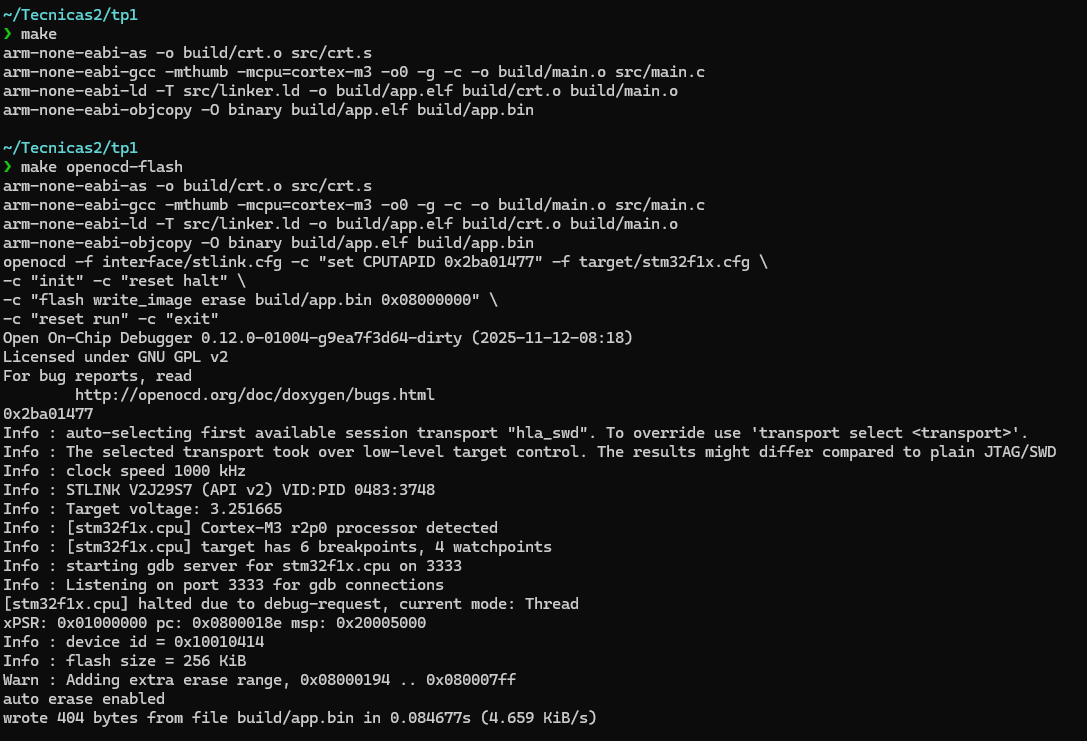
\includegraphics[width=0.5\textwidth]{images/compilacion.png}
    \caption*{Compilación del proyecto utilizando make}
    \label{fig:compilacion}
\end{figure}
Para el funcionamiento de la placa clon, se tuvieron que cambiar los comandos de programación y depuración, además de modificar el Makefile para añadir dichos comandos y así que funcione de manera correcta.